\documentclass[]{scrartcl}

%opening
\title{March Madness Analysis}
\author{Biased Estimators: Alexander Van Roijen, Molly Clark, Rocco Bavuso}
\usepackage[margin=1.0in]{geometry}
\usepackage{color}
\usepackage{times}
\usepackage[pdftex]{hyperref}


\setlength{\parindent}{0in}
\setlength{\parskip}{2ex}
\renewcommand{\baselinestretch}{1.0}

\usepackage{graphicx}
\usepackage{caption}
\usepackage{float}


\begin{document}

\maketitle

\begin{abstract}
\begin{center}
	\noindent March Madness is an annual NCAA Division I Basketball tournament. The tournament occurs in the month of March, thereby earning its name. There are 64 teams in the tournament each year, seeded into four regions that each contain 16 teams. This report will look at how far each team makes it into the tournament, based on their regular season data and prior tournament success.
\end{center}
\end{abstract}

\section*{Introduction}
\noindent In this report we work with data that was obtained from kaggle.com. We were interested to see what factors most affect a team's success in the March Madness tournament, so we compare teams to each other for every year that we have data. In doing so, we narrow down our predictors to find the best model of a team's success in the tournament for each year.

\noindent We were motivated to look into this data in part because the tournament is so hard to predict from year to year. We wondered what statistics and data from a team's season and history could be used to estimate how far the team would make it in the tournament. It is not uncommon for there to be many upsets over the course of the tournament, which can throw off any model, so we had to consider this uncertainty when choosing the best model.
\section*{Data Summary}
From Kaggle's website, we downloaded a data set that gave us a look at all Division I teams who did or did not qualify for the March Madness tournament in the past 30 or so years. Each team is assigned a four digit code that is consistent from season to season and data set to data set. This allows us to manipulate and analyze the data across the different files.

We had data that was collected during the regular season and data that was collected during the tournament, but in the long run choose to focus our model on regular season data so as to be able to predict the current season's tournament success if need be.

For the years 1985 to 2003, we have data in regards to the wins and losses of each involved team. For the years 2003 to 2016, we have more in depth data that includes each team's statistics from each game all season and throughout the tournament.

We began by looking at the data that has been collected season to season and follow up by looking at the data from previous tournaments and regional and past seed data to see which factors effect a team's chances of winning games in the tournament.

Because this tournament occurs each year, and because our data spans many years, we also saw it fitting to analyze how well teams had performed in the past when trying to predict their success in the future. The expectations and reputation of a team surely have an impact on how well they perform during the season and tournament, so temporal data about past success was essential to our model.

Throughout this report, let the following be universally true:

{\textbf {Field Goals:}} defined as any shot that is made in the game and is worth 2 points (within the 3 point line, not a free throw)

{\textbf {Three Pointers:}} defined as any shot that is made in the game and is worth 3 points (outside the 3 point line, from any place)

{\textbf {Free Throws:}} defined as any shot that is made in the game and is worth 1 point (shot after being fouled in any form, from the free throw line)

{\textbf {Assist:}} defined as a pass to another player who then immediately scores

{\textbf {Rebound:}} defined as a play in which a player grabs the ball, which bounced off of either the rim or backboard on an attempted shot. For this paper, we include offensive and defensive rebounds

{\textbf {Turnovers:}} defined as any action that results in the loss of basketball. (an action that gives the basketball to the other team not including a failed shot attempt)

{\textbf {Steals:}} defined as a defensive play in which a player steals the basketball from an opposing player

{\textbf {Block:}} defined as a defensive play in which a player deflects an opposing shot attempt before it reaches the basket

{\textbf {Personal Fouls:}} defined as an action that results in either a loss of possession or free throws for the other team
\section*{Pre-Analysis}
We began by looking at our data from a lens that based winning teams against losing teams. This was based on who won and lost each game of each season, so it is important to note that it is likely that teams would fall into both categories on occasion. We hoped to find what factors and variables in a season could predict a team's overall success in the tournament and moving forward.

We already had easy access to data that was parsed based on which team had won and which team had lost, so this seemed like a logical first step. We chose to keep regular season data apart from tournament data because the game play is so different in the tournament. In general, it is expected that the involved teams are among the best in the country, and the games have much higher stakes, so statistics may look different.
\subsection*{Regular Season Data}
In working with the regular season data, we first looked at some larger scale averages, comparing winning teams to losing teams on a very basic level.

We compared the average statistics of winning teams to the average statistics of losing teams and found what many would expect: on average, winning teams perform better in areas that are considered "good" statistics, whereas losing teams have higher rates of "bad" statistics.
\begin{figure}[H]
	\begin{center}
	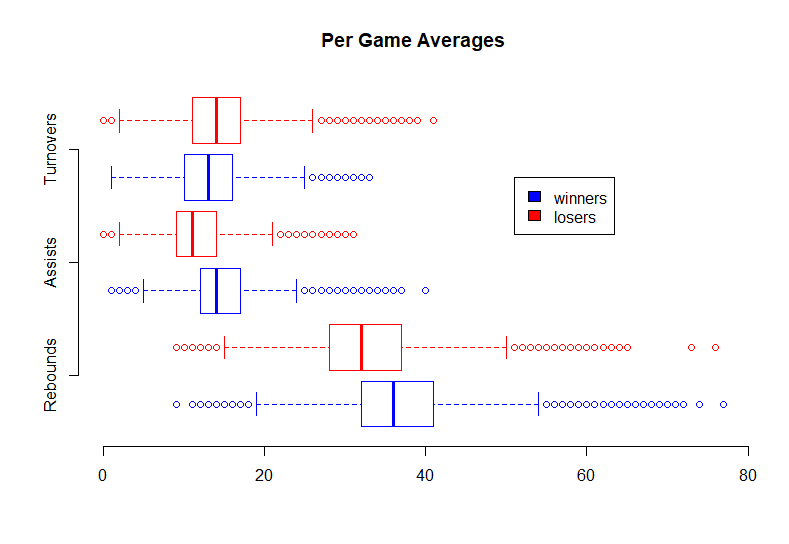
\includegraphics[scale=.4]{GameAverages.png}
	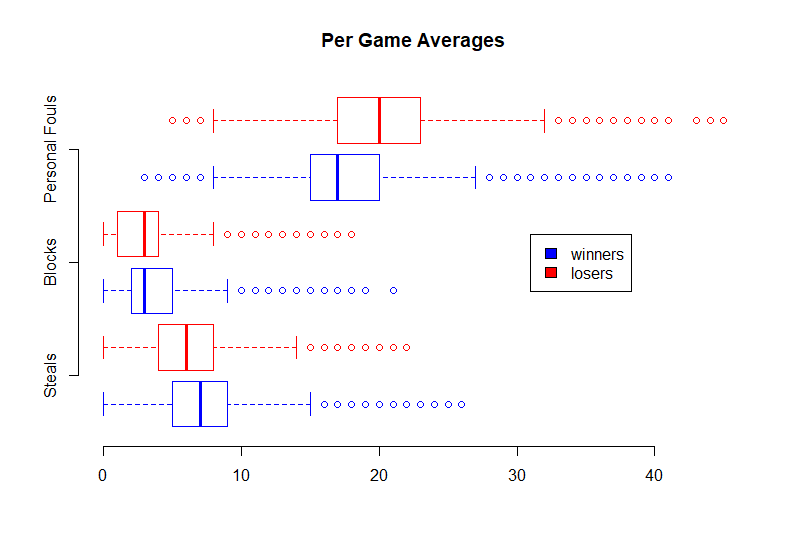
\includegraphics[scale=.4]{GameAverages2.png}
	\end{center}
\end{figure}
The above figures show the distribution of the winning and losing teams' averages throughout the years. They illustrate the above point that winning teams have higher averages in more beneficial statistics such as Rebounds, Assists, and Steals. This is a trend that we take note of when moving forward.

We then looked at winning and losing teams' average shooting percentages for the regular season. We were hoping to find which shots hold the most weight in the game. For example, three point shots are worth more points than any other shots, but free throws offer up an easy opportunity for a point or two and may be necessary late in the game.
\begin{figure}[H]
	\centering
	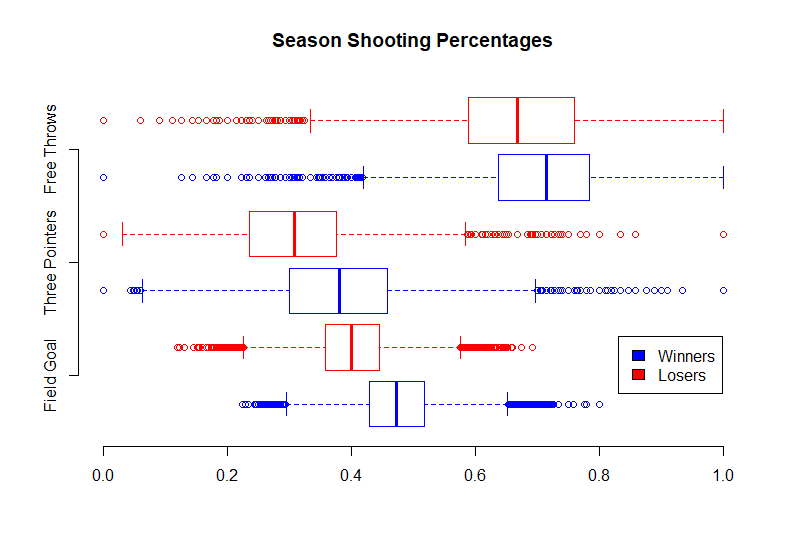
\includegraphics[scale=.5]{SeasonShotPercent.png}
\end{figure}
This figure visualizes the differences that exist, on average, in winning and losing teams' shot percentages. There are a large number of outliers in this plot, which should be noted for future analysis. It is also hard to tell which shots look to be more influential in the winning of a game because the data is so wide-spread.
\subsection*{Checking Parameters for Normality}
In order to test potential parameters for normality, we look at the QQ-plots. For field goal percentage, three point percentage, rebounds per game, and assists per game. Due to the large sample size, over 140,000, we do not anticiapte having issues due to the Central Limit Theorem.  
\begin{figure}[H]
	\centering
	\includegraphics[scale=.6]{FGnorm.pdf}
	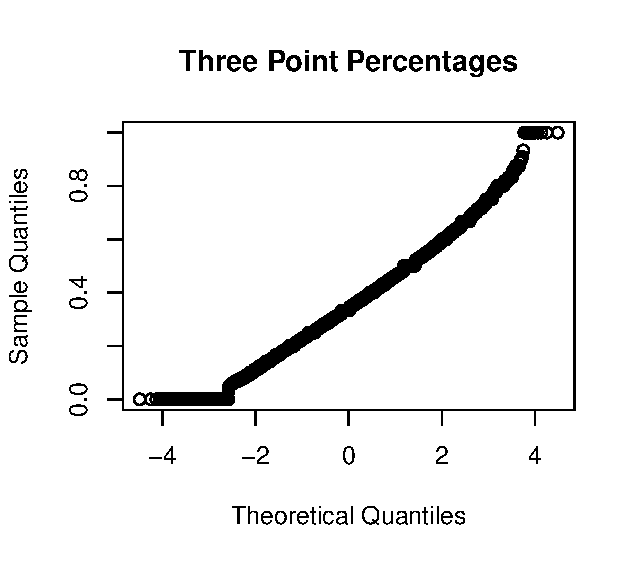
\includegraphics[scale=.6]{3pnorm.pdf}
	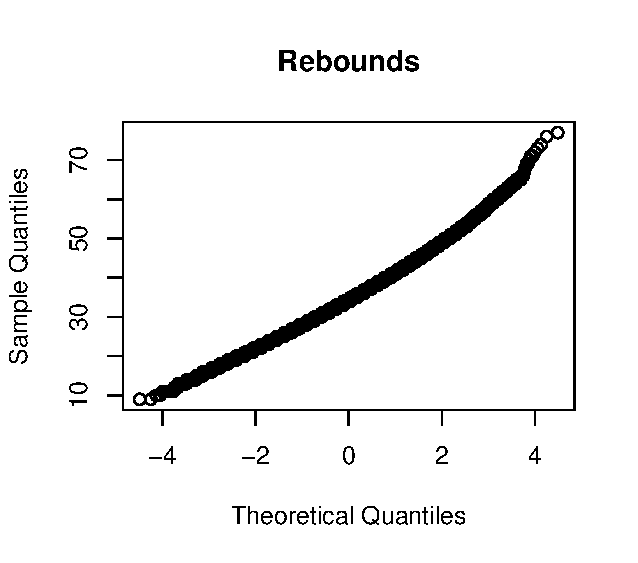
\includegraphics[scale=.6]{rbnorm.pdf}
	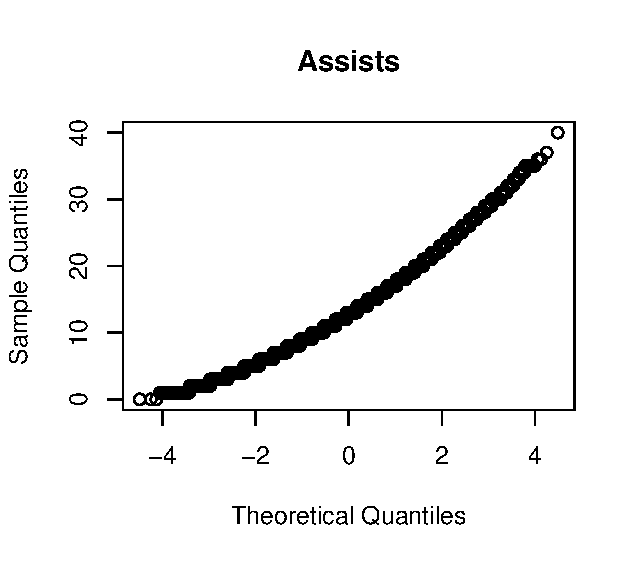
\includegraphics[scale=.6]{assnorm.pdf}
\end{figure}
The only parameter of concern here is the tails of the three point percentage. The minimum and maximum values of this value are 0 and 1, respectively. The issue here lies in the fact that there are several data points with these minimum and maximum values, but there is a gap of values just above the minimum and just below the maximum. For example, for a team to shoot 1 percent on three pointers, the team would have to only hit 1 and attempt 100. This is not plausible. However, a team can only attempt 5 three points and miss all of them, giving them a three point percentage of 0. The same analysis can be made for the maximum value. 
\subsection*{Tournament Data}
Much the same as when we worked with the regular season data, we analyzed the tournament data at first on a more basic level of winning teams versus losing teams. Much of the data that we had for tournaments was centered on the teams' abilities to score. We analyzed their shooting percentages during the tournaments and compared average winning teams to average losing teams.
\begin{figure}[H]
	\centering
	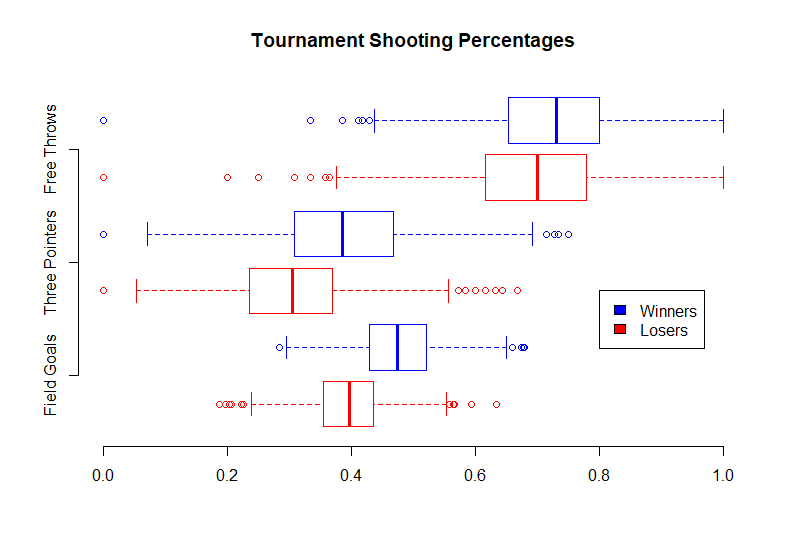
\includegraphics[scale=.5]{TourneyShotPercent.png}
\end{figure}
As the above figure illustrates, winning teams, on average, have higher shooting percentages in all categories. It is essential to note how large the differences may be. From this data we can start to decide which types of shots are the most important to tournament success.
\subsection*{History of Success}
As a result of looking at our data, and through our own personal knowledge of the sport, we decided it was fitting to look into each team's history of success in the tournament and how often they had been seeded near the top.
\begin{figure}[H]
	\centering
	\includegraphics[scale=.5]{overLeaders.pdf}
\end{figure}
The above figure maps how often teams have been seeded among the top four, for any region in the tournament. Teams that have been successful in the past are more likely to be seeded near the top again in the future, as is pictured above. The teams near the top of this chart are those that are commonly discussed amongst basketball fans. They are teams that come from schools that are known for basketball, and they likely draw in more talented players as a result of their reputation, helping them further develop their program.

We continue this analysis of History of Success by looking at teams that are all-around leaders in past tournaments. We look at each team's past appearances in the tournament to compare them to each other.
\begin{figure}[H]
	\centering
	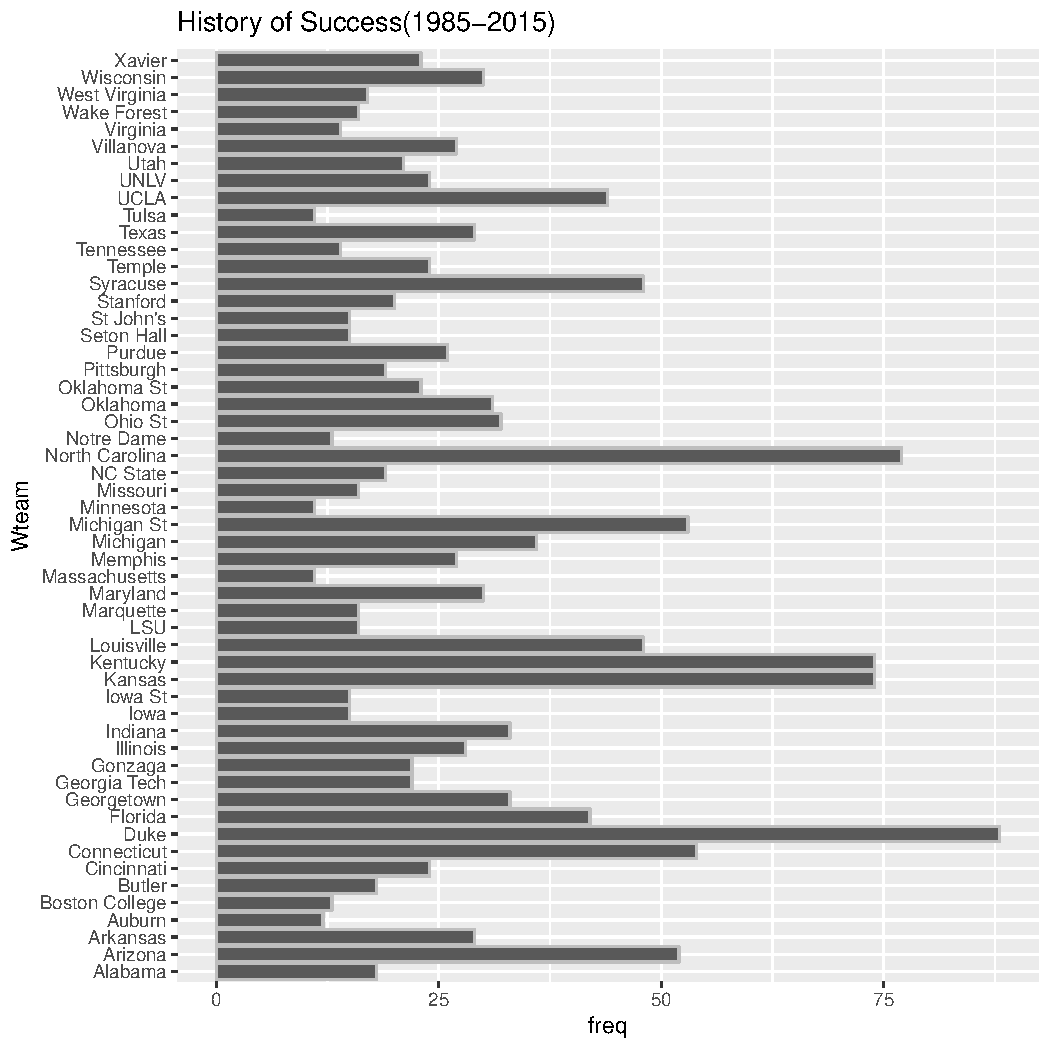
\includegraphics[scale=.5]{HistOfSuccess2.pdf}
\end{figure}
The figure above shows some of the teams with the most appearances in the March Madness tournament. Higher frequency logically relates to a better team, and this data allows us to see which teams are consistently present and performing in the tournament.

\section*{Initial Model}
	\[
Y_{daynum} = \beta_0 + \beta_{conf} + \beta_{fgp} +\beta_{tpp} + \beta_{ass} + \beta_{rb} + \beta_{app} + \epsilon
\]
Our original model contained all of the predictors that we felt would be the most important moving forward. These predictors and subscripts are outlined below:
	\begin{itemize}
	\item The response variable, {\textit{daynum}}, signifies what day of the year the last game is played for each team. This is a good measure of two things: If a team makes the tournament and how far that team advances.
	\item 	{\textit{conf:}} the conference the team plays in - different conferences have vastly different quality of teams
	\item 	{\textit{fgp:}} refers to field goal percentage
	\item 	{\textit{tpp:}} three point shooting percentage
	\item 	{\textit{ass:}} assists
	\item 	{\textit{rb:}} rebounds
	\item 	{\textit{app:}} prior tournament success - indicated by number of previous appearances in the tournament
	\end{itemize}
Seed is not included because seeding is almost entirely determined by conference and record. Record is left out because it is in large part determined by a teams statistics, which we have included in the model.
\section*{Processing}
In working with our data to develop a model, we realized that there may be a better way to interpret it. We also ran into problems with some predictors and variables because they were quite difficult to quantify or compare.

We found that {\textit{daynum}} may not be the best measure of a team's success in the tournament because the respective games of a tournament are played on slightly different days each year. This means that the team who won the tournament in 2003 could have a higher daynum than the team who won the tournament in 2004, automatically ranking the 2003 team higher, although they played and won the same number of games.

We also found that {\textit{conf}} was difficult to quantify because while some conferences are undoubtedly better than others, it is not up to our judgment as to decide how much better they are and which conferences deserve to be credited as the best.
\subsection*{Data Plumbing}
\subsection*{Data Reconstruction}
\section*{Full Model}
	\[
Y_{GP_{year}} = \beta_0 + \beta_{avgScore} + \beta_{avgASS} +\beta_{avgFT} + \beta_{avgPF} + \beta_{avgTP} + \beta_{avgRB} + \beta_{avgTO}
\] 
\[
+ \beta_{avgSTL} +\beta_{avgBL} + \beta_{GP_{year-1}}+ \epsilon
\]
We fit a full model with all of the possible predictors that we pulled from the data. The full list of predictors includes:
	\begin{itemize}
	\item 	{$GP_{year}$:} number of games the team plays in the tournament in a given year
	\item 	{\textit{avgScore:}} average score per team per game in regular season
	\item 	{\textit{avgASS:}} average assists per team per game in regular season
	\item 	{\textit{avgFT:}} average free throws per team per game in regular season
	\item 	{\textit{avgPF:}} average personal fouls per team per game in regular season
	\item 	{\textit{avgTP:}} average three point shots made per team per game in regular season
	\item 	{\textit{avgRB:}} average total rebounds per team per game in regular season
	\item 	{\textit{avgTO:}} average turnovers per team per game in regular season
	\item 	{\textit{avgSTL:}} average steals per team per game in regular season
	\item 	{\textit{avgBL:}} average blocks per team per game in regular season
	\item 	{$GP_{year-1}$:} number of games the team plays in the tournament in the prior year
	\end{itemize}
We formed this model for each year from 2004 to 2015 because those are the years that we have the most data for, and we seek out the model with the highest $R^{2}$ value because it accounts for the most variation in the response. The coefficients and summary of some of the models are shown below:
\footnotesize
\begin{verbatim}
> prev4 = addPriorYear(2,avgsZ,TRUE)
> fit04 = lm(GP04~.,prev4[,-1])
> summary(fit04)

Call:
lm(formula = GP04 ~ ., data = prev4[, -1])

Residuals:
    Min      1Q  Median      3Q     Max 
-1.7484 -0.6289 -0.1841  0.5283  3.5693 

Coefficients: (1 not defined because of singularities)
Estimate Std. Error t value Pr(>|t|)  
(Intercept) -2.476693   2.445436  -1.013   0.3157  
avgScore04  -0.003557   0.084844  -0.042   0.9667  
avgFG04      0.208241   0.238282   0.874   0.3860  
avgTP04      0.111249   0.147521   0.754   0.4541  
avgFT04            NA         NA      NA       NA  
avgRB04      0.011671   0.018473   0.632   0.5302  
avgASS04    -0.128551   0.119710  -1.074   0.2877  
avgTO04     -0.239030   0.112035  -2.134   0.0374 *
avgSTL04    -0.124997   0.123520  -1.012   0.3161  
avgBL04      0.328675   0.133100   2.469   0.0167 *
avgPF04      0.162716   0.105641   1.540   0.1293  
GP03         0.076130   0.112047   0.679   0.4998  
---
Signif. codes:  0 ‘***’ 0.001 ‘**’ 0.01 ‘*’ 0.05 ‘.’ 0.1 ‘ ’ 1

Residual standard error: 1.125 on 54 degrees of freedom
Multiple R-squared:  0.3546,	Adjusted R-squared:  0.2351 
F-statistic: 2.967 on 10 and 54 DF,  p-value: 0.004799

>
> prev9 = addPriorYear(7,avgsZ,TRUE)
> fit09 = lm(GP09~.,prev9[,-1])
> summary(fit09)

Call:
lm(formula = GP09 ~ ., data = prev9[, -1])

Residuals:
    Min      1Q  Median      3Q     Max 
-1.6153 -0.6350 -0.1082  0.5441  2.6755 

Coefficients: (1 not defined because of singularities)
Estimate Std. Error t value Pr(>|t|)    
(Intercept) -0.17350    2.63262  -0.066 0.947699    
avgScore09   0.22102    0.06561   3.369 0.001400 ** 
avgFG09     -0.59909    0.19117  -3.134 0.002789 ** 
avgTP09     -0.39458    0.12390  -3.185 0.002407 ** 
avgFT09           NA         NA      NA       NA    
avgRB09      0.01778    0.01539   1.155 0.253025    
avgASS09     0.34903    0.10525   3.316 0.001636 ** 
avgTO09     -0.03090    0.10399  -0.297 0.767497    
avgSTL09     0.19539    0.12018   1.626 0.109797    
avgBL09     -0.08933    0.11806  -0.757 0.452553    
avgPF09     -0.15114    0.10048  -1.504 0.138351    
GP08         0.28387    0.07955   3.568 0.000763 ***
---
Signif. codes:  0 ‘***’ 0.001 ‘**’ 0.01 ‘*’ 0.05 ‘.’ 0.1 ‘ ’ 1

Residual standard error: 0.9419 on 54 degrees of freedom
Multiple R-squared:  0.5478,	Adjusted R-squared:  0.4641 
F-statistic: 6.542 on 10 and 54 DF,  p-value: 1.58e-06

>
> prev15 = addPriorYear(13,avgsZ,TRUE)
> fit15 = lm(GP15~.,prev15[,-1])
> summary(fit15)

Call:
lm(formula = GP15 ~ ., data = prev15[, -1])

Residuals:
    Min       1Q   Median       3Q      Max 
-2.13475 -0.74144 -0.07461  0.59031  2.93999 

Coefficients: (1 not defined because of singularities)
Estimate Std. Error t value Pr(>|t|)    
(Intercept) -1.137942   2.505740  -0.454  0.65146    
avgScore15   0.009128   0.087329   0.105  0.91712    
avgFG15      0.222098   0.204176   1.088  0.28127    
avgTP15     -0.161144   0.132683  -1.215  0.22956    
avgFT15            NA         NA      NA       NA    
avgRB15      0.018762   0.013055   1.437  0.15615    
avgASS15    -0.062710   0.100166  -0.626  0.53378    
avgTO15     -0.156939   0.122918  -1.277  0.20686    
avgSTL15     0.055784   0.118423   0.471  0.63940    
avgBL15     -0.035234   0.118800  -0.297  0.76787    
avgPF15     -0.042033   0.082793  -0.508  0.61363    
GP14         0.372234   0.099741   3.732  0.00044 ***
---
Signif. codes:  0 ‘***’ 0.001 ‘**’ 0.01 ‘*’ 0.05 ‘.’ 0.1 ‘ ’ 1

Residual standard error: 1.011 on 57 degrees of freedom
Multiple R-squared:  0.4606,	Adjusted R-squared:  0.366 
F-statistic: 4.868 on 10 and 57 DF,  p-value: 4.65e-05
\end{verbatim}
\normalsize
The above code output shows the coefficients for three models, from years 2004, 2009, and 2015. Clearly, the $R^{2}$ values vary from model to model, but we found that the model from 2009 had the highest $R^{2}$ value and the most significant figures when compared to the other full models.
\section*{Full Model Analysis}
We were clearly working with too many predictors in the full model, so we ran diagnostic tests on the full 2009 model and then used the stepwise function, both forward and backward, to reduce the number of predictors. We decided to start by working with the 2009 model because it had a high $R^{2}$ value and many significant predictors.
\footnotesize
\begin{verbatim}
plot(fitted(fit09), residuals(fit09))
abline(h=0)
\end{verbatim}
\normalsize
\begin{figure}[H]
	\centering
	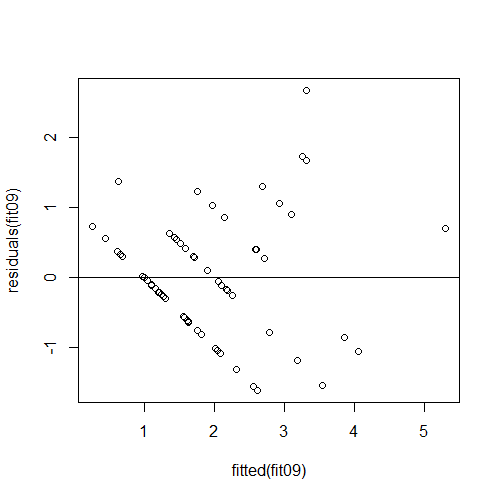
\includegraphics[scale=.6]{2009resid.png}
\end{figure}
Clearly, there is a distinct fan shape to our residual plot, so we ran a boxcox function to see what type of transformation we should perform on the data.
\footnotesize
\begin{verbatim}
boxcox(fit09, plotit = TRUE)
\end{verbatim}
\normalsize
\begin{figure}[H]
	\centering
	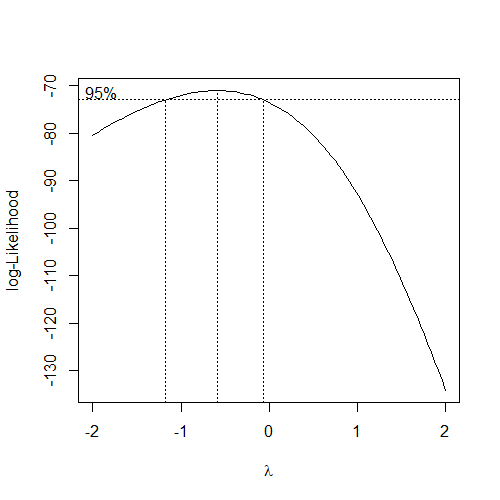
\includegraphics[scale=.6]{2009box.png}
\end{figure}
The boxcox graph shows that we should raise the response to the -$\frac{1}{2}$, so we adjust the model and re-plot the residuals.
\footnotesize
\begin{verbatim}
fit09Adj <- lm(I(GP09^(-1/2))~.,prev9[,-1])
plot(fitted(fit09Adj), residuals(fit09Adj))
abline(h=0)
summary(fit09Adj)

Output:
Call:
lm(formula = I(GP09^(-1/2)) ~ ., data = prev9[, -1])

Residuals:
Min        1Q    Median        3Q       Max 
-0.295461 -0.131892  0.006337  0.113975  0.282223 

Coefficients: (1 not defined because of singularities)
Estimate Std. Error t value Pr(>|t|)    
(Intercept)  0.623708   0.440643   1.415 0.162678    
avgScore09  -0.033851   0.010982  -3.082 0.003231 ** 
avgFG09      0.091291   0.031998   2.853 0.006127 ** 
avgTP09      0.066538   0.020738   3.208 0.002246 ** 
avgFT09            NA         NA      NA       NA    
avgRB09     -0.001131   0.002575  -0.439 0.662340    
avgASS09    -0.038591   0.017616  -2.191 0.032810 *  
avgTO09      0.016290   0.017406   0.936 0.353500    
avgSTL09    -0.046625   0.020115  -2.318 0.024271 *  
avgBL09      0.020326   0.019761   1.029 0.308254    
avgPF09      0.031443   0.016818   1.870 0.066959 .  
GP08        -0.051046   0.013315  -3.834 0.000332 ***
---
Signif. codes:  0 ‘***’ 0.001 ‘**’ 0.01 ‘*’ 0.05 ‘.’ 0.1 ‘ ’ 1

Residual standard error: 0.1576 on 54 degrees of freedom
Multiple R-squared:  0.5097,	Adjusted R-squared:  0.4189 
F-statistic: 5.614 on 10 and 54 DF,  p-value: 1.074e-05
\end{verbatim}
\normalsize
\begin{figure}[H]
	\centering
	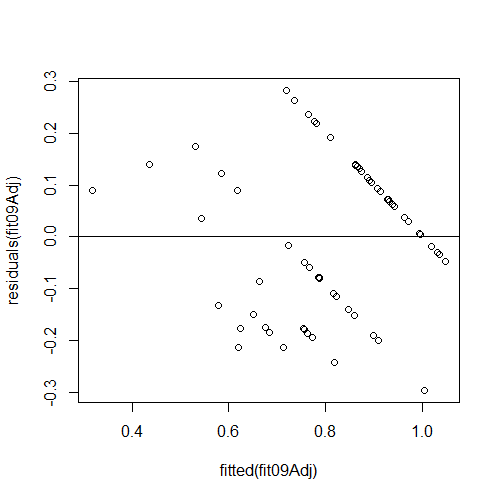
\includegraphics[scale=.6]{2009Aresid.png}
\end{figure}
The residual plot is not perfect, but they are more evenly spaced from 0, so we move forward with the adjusted model.

We continue by testing the normality of the residuals.
\footnotesize
\begin{verbatim}
qqnorm(fit09Adj$residuals)
\end{verbatim}
\normalsize
\begin{figure}[H]
	\centering
	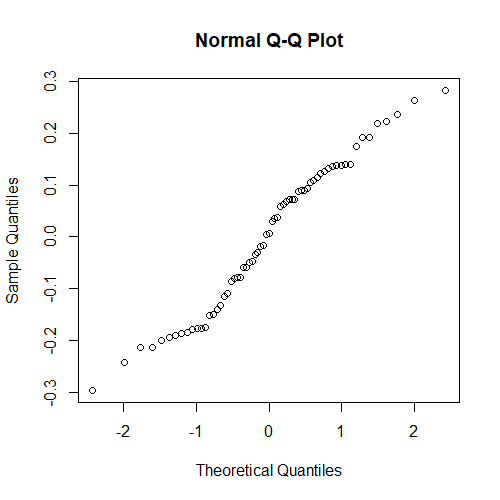
\includegraphics[scale=.6]{2009Anorm.png}
\end{figure}
The residuals seem to follow a fairly Normal pattern, so we continue to move forward.
\section*{Final Model}
	\[
Y_{GP_{year}}^{-0.5} = \beta_0 + \beta_{avgASS} +\beta_{avgFT} + \beta_{avgPF} + \beta_{avgFG} + \beta_{avgTO} + \beta_{GP_{year-1}}+ \epsilon 
\]
\section*{Final Model Analysis}
Each predictor in the final model carries significant meaning with valuable interpretation. Average assists, free throws and field goals measure overall offensive power, while turnovers measures how careful the offense is. Assist to turnover ratio was found to be ineffective as this data variable was not distinguishable enough from team to team. Generally, the more assists a team has the more ball movement they have, the more prone they are to turning the ball over. Amongst March Madness bracket teams, the individual number of assists and turnovers proved to be more of a relevant statistic than assist to turnover ratio. Furthermore, the assist to turnover ratio is more precise and valuable in measuring a particular players effectiveness, for example a team's point guard. The remaining predictors are personal fouls and prior year success. Personal fouls is a measure of a team's defensive ability. This is not the best statistic for measuring a teams defensive capability, but it is for this data set. Prior year tournament success is the last predictor and is the most straight forward. There is tremendous correlation across time for teams making the tournament one year if they made it the previous year.

We ran the summary function on this model and the output is shown below:
\footnotesize
\begin{verbatim}
> fit09Adj2 = lm(GP09~GP08+avgASS09+avgFT09+avgPF09+avgSTL09+avgScore09,prev9[,-1])
> summary(fit09Adj2)

Call:
lm(formula = GP09 ~ GP08 + avgASS09 + avgFT09 + avgPF09 + avgSTL09 + 
avgScore09, data = prev9[, -1])

Residuals:
Min       1Q   Median       3Q      Max 
-1.61295 -0.70409 -0.09138  0.48096  2.81927 

Coefficients:
Estimate Std. Error t value Pr(>|t|)    
(Intercept) -1.14986    2.38317  -0.482 0.631271    
GP08         0.28555    0.07462   3.826 0.000321 ***
avgASS09     0.36007    0.10294   3.498 0.000908 ***
avgFT09      0.32947    0.08863   3.717 0.000455 ***
avgPF09     -0.14265    0.08185  -1.743 0.086682 .  
avgSTL09     0.18756    0.11075   1.694 0.095708 .  
avgScore09  -0.08360    0.04462  -1.873 0.066046 .  
---
Signif. codes:  0 ‘***’ 0.001 ‘**’ 0.01 ‘*’ 0.05 ‘.’ 0.1 ‘ ’ 1

Residual standard error: 0.9317 on 58 degrees of freedom
Multiple R-squared:  0.5247,	Adjusted R-squared:  0.4755 
F-statistic: 10.67 on 6 and 58 DF,  p-value: 5.829e-08
\end{verbatim}
\normalsize
This model has an Adjusted $R^{2}$ of 0.4755, which is a higher than the full 2009 model, and it contains the predictors that were seen most often in all of the years of data. Three predictors and the intercept are significant in this model. This model explains the most variation and contains predictors that encompass all of the models, so it is out choice moving forward.
\section*{Predictions}
We used our model to predict for two teams to test it's predictive power. We tested for Duke and Albany.
\footnotesize
\begin{verbatim}
Duke:
> predict(fit09Adj2, predset09, interval="predict")
       fit      lwr      upr
  3.145849 1.042621 5.249077
  
Albany
> predict(fit09Adj2, predset, interval="predict")
       fit       lwr      upr
  2.189929 0.2506521 4.129206
\end{verbatim}
\normalsize
It turned out that these predictions were fairly accurate for Duke, who played 3 games in the 2009 season, although the prediction was a little off for Albany, who didn't make the tournament in the 2009 season.

We found that our model was better at predicting for teams who frequently make the tournament. In the above example, both teams had similar stats, aside from games played in the previous season. However, if teams do not often show, they are seeded lower and are often less likely to progress in the tournament. This could be due to a number of things: the teams have more experience playing in high stakes games, they are more popular and able to recruit talented, young players, they may have more consistent coaching staff to work with, etc.

\section*{Further Research}
Further research that would likely have more prediction power would incorporate advanced sports statistics. The most important improvement in the model could be defensive metrics. As far as stat sheet statistics go for defense, the only measurable statistics are bocks, steals, and personal fouls. Blocks and steals do not occur many times in a game, the  player that leads the league in either category typically does not average more than four per game. In the past ten years, a great deal of advancements in statistical analysis have paved the way for new defensive metrics for a basketball team. A common statistic is points allowed per 100 possessions. The team with the fewest points allowed per 100 possessions would be classified as the team with the lowest scoring defense. Unfortunately, in our data set, we could not formulate any advanced defensive statistics.

Another predictor we would like to have in the future is a measure of conference. This was expressed in our initial, hypothetical model but not in our final model. In NCAA basketball, specific conferences have more high quality teams. These teams are more likely to make the tournament even if their record is inferior to other teams in other conferences. There are a total of 32 conferences for the 2017-2018 season, but only 7 of them make up the majority of NCAA tournament teams: Big 12, ACC, Big East, Big Ten, SEC, The American, and the Pac-12. Every  year multiple teams from these conferences make the tournament. This cannot be said for all conferences. For example, Binghamton's basketball team lies in the American East conference. Only the winner of this conference typically makes the tournament. Future models should incorporate some kind of dummy variable to account for this variation. A predictor variable "conference" could be added. Teams in these conferences would be assigned a value of 1 while other teams would be assigned a value of zero. This would help the prediction of the model, due to the fact that two teams in different conferences can have very similar statistics on paper, but one will make the tournament and one will not. A good example of this was this year's Vermont team in the American East conference. Vermont had a 27-8 overall record, but failed to make the NCAA tournament due to their loss in the American East tournament. Teams with this record in the seven conferences previously mentioned would make the NCAA tournament every year. Only one team in the modern NCAA tournament era, 1985-present, won the tournament outside of these seven conferences, which was UNLV in 1990. Interestingly enough, three players from this team were selected in the first 12 picks of the NBA draft the next year, including the number one overall pick.   
\section*{Appendix}
{\textbf{Summary output for full model:}}
\footnotesize
\begin{verbatim}
> prev14 = addPriorYear(12,avgsZ,TRUE)
> fit14 = lm(GP14~.,prev14[,-1])
> summary(fit14)

Call:
lm(formula = GP14 ~ ., data = prev14[, -1])

Residuals:
    Min      1Q  Median      3Q     Max 
-1.6535 -0.6375 -0.1490  0.3945  3.7843 

Coefficients: (1 not defined because of singularities)
Estimate Std. Error t value Pr(>|t|)  
(Intercept)  5.301180   2.745766   1.931   0.0585 .
avgScore14  -0.104674   0.083860  -1.248   0.2171  
avgFG14      0.309636   0.239501   1.293   0.2013  
avgTP14      0.156841   0.153644   1.021   0.3117  
avgFT14            NA         NA      NA       NA  
avgRB14      0.009232   0.018780   0.492   0.6249  
avgASS14    -0.053165   0.107422  -0.495   0.6226  
avgTO14     -0.209756   0.127291  -1.648   0.1049  
avgSTL14    -0.145048   0.133040  -1.090   0.2802  
avgBL14      0.275043   0.145680   1.888   0.0641 .
avgPF14     -0.106358   0.110073  -0.966   0.3380  
GP13         0.082681   0.126693   0.653   0.5166  
---
Signif. codes:  0 ‘***’ 0.001 ‘**’ 0.01 ‘*’ 0.05 ‘.’ 0.1 ‘ ’ 1

Residual standard error: 1.208 on 57 degrees of freedom
Multiple R-squared:  0.2437,	Adjusted R-squared:  0.1111 
F-statistic: 1.837 on 10 and 57 DF,  p-value: 0.07443

> 
> prev13 = addPriorYear(11,avgsZ,TRUE)
> fit13 = lm(GP13~.,prev13[,-1])
> summary(fit13)

Call:
lm(formula = GP13 ~ ., data = prev13[, -1])

Residuals:
    Min      1Q  Median      3Q     Max 
-1.8786 -0.6606 -0.1628  0.5599  3.1439 

Coefficients: (1 not defined because of singularities)
Estimate Std. Error t value Pr(>|t|)  
(Intercept)  3.30169    3.04878   1.083   0.2834  
avgScore13  -0.06515    0.09446  -0.690   0.4932  
avgFG13      0.20597    0.23302   0.884   0.3805  
avgTP13      0.08966    0.15024   0.597   0.5530  
avgFT13           NA         NA      NA       NA  
avgRB13      0.01222    0.02041   0.599   0.5516  
avgASS13    -0.14487    0.11411  -1.270   0.2094  
avgTO13     -0.04789    0.12670  -0.378   0.7068  
avgSTL13     0.29211    0.13630   2.143   0.0364 *
avgBL13      0.01784    0.14977   0.119   0.9056  
avgPF13     -0.16485    0.12234  -1.347   0.1832  
GP12         0.25061    0.11103   2.257   0.0279 *
---
Signif. codes:  0 ‘***’ 0.001 ‘**’ 0.01 ‘*’ 0.05 ‘.’ 0.1 ‘ ’ 1

Residual standard error: 1.154 on 57 degrees of freedom
Multiple R-squared:  0.3101,	Adjusted R-squared:  0.1891 
F-statistic: 2.562 on 10 and 57 DF,  p-value: 0.01243

> 
> prev12 = addPriorYear(10,avgsZ,TRUE)
> fit12 = lm(GP12~.,prev12[,-1])
> summary(fit12)

Call:
lm(formula = GP12 ~ ., data = prev12[, -1])

Residuals:
    Min      1Q  Median      3Q     Max 
-2.3717 -0.6724 -0.1912  0.4705  2.8825 

Coefficients: (1 not defined because of singularities)
Estimate Std. Error t value Pr(>|t|)   
(Intercept)  3.58332    2.81280   1.274  0.20786   
avgScore12  -0.17995    0.08624  -2.087  0.04141 * 
avgFG12      0.36211    0.25401   1.426  0.15945   
avgTP12      0.01410    0.13270   0.106  0.91576   
avgFT12           NA         NA      NA       NA   
avgRB12      0.06054    0.02019   2.999  0.00402 **
avgASS12    -0.06248    0.13882  -0.450  0.65437   
avgTO12     -0.01225    0.11686  -0.105  0.91686   
avgSTL12     0.10954    0.12354   0.887  0.37899   
avgBL12      0.07202    0.15598   0.462  0.64602   
avgPF12     -0.04097    0.10304  -0.398  0.69239   
GP11         0.22083    0.10731   2.058  0.04419 * 
---
Signif. codes:  0 ‘***’ 0.001 ‘**’ 0.01 ‘*’ 0.05 ‘.’ 0.1 ‘ ’ 1

Residual standard error: 1.075 on 57 degrees of freedom
Multiple R-squared:  0.3898,	Adjusted R-squared:  0.2827 
F-statistic: 3.641 on 10 and 57 DF,  p-value: 0.0008516

> 
> prev11 = addPriorYear(9,avgsZ,TRUE)
> fit11 = lm(GP11~.,prev11[,-1])
> summary(fit11)

Call:
lm(formula = GP11 ~ ., data = prev11[, -1])

Residuals:
    Min      1Q  Median      3Q     Max 
-1.5599 -0.7117 -0.3055  0.4825  4.0113 

Coefficients: (1 not defined because of singularities)
Estimate Std. Error t value Pr(>|t|)  
(Intercept)  2.261465   2.888834   0.783   0.4370  
avgScore11  -0.007744   0.092958  -0.083   0.9339  
avgFG11      0.256092   0.263395   0.972   0.3350  
avgTP11      0.162204   0.166759   0.973   0.3348  
avgFT11            NA         NA      NA       NA  
avgRB11      0.013038   0.018242   0.715   0.4777  
avgASS11    -0.293256   0.135765  -2.160   0.0350 *
avgTO11     -0.046868   0.145977  -0.321   0.7493  
avgSTL11     0.108027   0.140027   0.771   0.4436  
avgBL11      0.014608   0.162108   0.090   0.9285  
avgPF11     -0.223840   0.124075  -1.804   0.0765 .
GP10         0.151927   0.102938   1.476   0.1455  
---
Signif. codes:  0 ‘***’ 0.001 ‘**’ 0.01 ‘*’ 0.05 ‘.’ 0.1 ‘ ’ 1

Residual standard error: 1.201 on 57 degrees of freedom
Multiple R-squared:  0.2788,	Adjusted R-squared:  0.1523 
F-statistic: 2.204 on 10 and 57 DF,  p-value: 0.03038

> 
> prev10 = addPriorYear(8,avgsZ,TRUE)
> fit10 = lm(GP10~.,prev10[,-1])
> summary(fit10)

Call:
lm(formula = GP10 ~ ., data = prev10[, -1])

Residuals:
    Min      1Q  Median      3Q     Max 
-1.6940 -0.7676 -0.3351  0.5501  3.7452 

Coefficients: (1 not defined because of singularities)
Estimate Std. Error t value Pr(>|t|)  
(Intercept)  1.40279    3.22112   0.435   0.6649  
avgScore10   0.07318    0.09513   0.769   0.4451  
avgFG10     -0.26524    0.25676  -1.033   0.3062  
avgTP10      0.01756    0.19928   0.088   0.9301  
avgFT10           NA         NA      NA       NA  
avgRB10      0.01787    0.01944   0.919   0.3620  
avgASS10     0.05366    0.12805   0.419   0.6768  
avgTO10     -0.07381    0.14292  -0.516   0.6077  
avgSTL10    -0.10435    0.13868  -0.752   0.4551  
avgBL10      0.28555    0.17057   1.674   0.0999 .
avgPF10      0.03564    0.11033   0.323   0.7479  
GP09         0.26721    0.11937   2.239   0.0293 *
---
Signif. codes:  0 ‘***’ 0.001 ‘**’ 0.01 ‘*’ 0.05 ‘.’ 0.1 ‘ ’ 1

Residual standard error: 1.257 on 54 degrees of freedom
Multiple R-squared:  0.1949,	Adjusted R-squared:  0.04579 
F-statistic: 1.307 on 10 and 54 DF,  p-value: 0.2504

> 
> prev8 = addPriorYear(6,avgsZ,TRUE)
> fit08 = lm(GP08~.,prev8[,-1])
> summary(fit08)

Call:
lm(formula = GP08 ~ ., data = prev8[, -1])

Residuals:
    Min       1Q   Median       3Q      Max 
-1.42411 -0.62107 -0.08825  0.63471  1.95409 

Coefficients: (1 not defined because of singularities)
Estimate Std. Error t value Pr(>|t|)    
(Intercept) -1.38585    2.00584  -0.691  0.49258    
avgScore08  -0.02949    0.07537  -0.391  0.69716    
avgFG08      0.16887    0.18739   0.901  0.37152    
avgTP08     -0.24737    0.12896  -1.918  0.06039 .  
avgFT08           NA         NA      NA       NA    
avgRB08      0.03838    0.01563   2.456  0.01730 *  
avgASS08     0.03256    0.09736   0.334  0.73936    
avgTO08     -0.23483    0.09382  -2.503  0.01537 *  
avgSTL08     0.09159    0.10375   0.883  0.38123    
avgBL08      0.06124    0.10269   0.596  0.55342    
avgPF08      0.14675    0.09236   1.589  0.11792    
GP07         0.33183    0.08974   3.698  0.00051 ***
---
Signif. codes:  0 ‘***’ 0.001 ‘**’ 0.01 ‘*’ 0.05 ‘.’ 0.1 ‘ ’ 1

Residual standard error: 0.9184 on 54 degrees of freedom
Multiple R-squared:  0.5701,	Adjusted R-squared:  0.4905 
F-statistic:  7.16 on 10 and 54 DF,  p-value: 4.689e-07

> 
> prev7 = addPriorYear(5,avgsZ,TRUE)
> fit07 = lm(GP07~.,prev7[,-1])
> summary(fit07)

Call:
lm(formula = GP07 ~ ., data = prev7[, -1])

Residuals:
    Min      1Q  Median      3Q     Max 
-1.7748 -0.7216 -0.2807  0.6634  2.4802 

Coefficients: (1 not defined because of singularities)
Estimate Std. Error t value Pr(>|t|)   
(Intercept)  2.6029631  2.4564810   1.060  0.29403   
avgScore07  -0.0651920  0.0718252  -0.908  0.36810   
avgFG07      0.2446843  0.1938464   1.262  0.21228   
avgTP07      0.1423438  0.1418684   1.003  0.32017   
avgFT07             NA         NA      NA       NA   
avgRB07     -0.0005477  0.0172239  -0.032  0.97475   
avgASS07     0.0260457  0.1167849   0.223  0.82436   
avgTO07     -0.2402723  0.0966838  -2.485  0.01608 * 
avgSTL07    -0.0466975  0.1167059  -0.400  0.69064   
avgBL07      0.1657333  0.1212501   1.367  0.17733   
avgPF07     -0.0462716  0.0882245  -0.524  0.60209   
GP06         0.3212087  0.1051509   3.055  0.00349 **
---
Signif. codes:  0 ‘***’ 0.001 ‘**’ 0.01 ‘*’ 0.05 ‘.’ 0.1 ‘ ’ 1

Residual standard error: 1.056 on 54 degrees of freedom
Multiple R-squared:  0.4317,	Adjusted R-squared:  0.3265 
F-statistic: 4.102 on 10 and 54 DF,  p-value: 0.0003138

> 
> prev6 = addPriorYear(4,avgsZ,TRUE)
> fit06 = lm(GP06~.,prev6[,-1])
> summary(fit06)

Call:
lm(formula = GP06 ~ ., data = prev6[, -1])

Residuals:
    Min      1Q  Median      3Q     Max 
-1.6347 -0.8841 -0.2856  0.5480  4.1550 

Coefficients: (1 not defined because of singularities)
Estimate Std. Error t value Pr(>|t|)  
(Intercept)  0.205358   2.752568   0.075   0.9408  
avgScore06   0.076930   0.095801   0.803   0.4255  
avgFG06      0.017233   0.261605   0.066   0.9477  
avgTP06     -0.005185   0.164894  -0.031   0.9750  
avgFT06            NA         NA      NA       NA  
avgRB06     -0.014477   0.017667  -0.819   0.4161  
avgASS06    -0.055950   0.131938  -0.424   0.6732  
avgTO06      0.030397   0.141820   0.214   0.8311  
avgSTL06     0.046671   0.123428   0.378   0.7068  
avgBL06      0.133624   0.139198   0.960   0.3414  
avgPF06     -0.232631   0.114706  -2.028   0.0475 *
GP05         0.017416   0.106412   0.164   0.8706  
---
Signif. codes:  0 ‘***’ 0.001 ‘**’ 0.01 ‘*’ 0.05 ‘.’ 0.1 ‘ ’ 1

Residual standard error: 1.235 on 54 degrees of freedom
Multiple R-squared:  0.2222,	Adjusted R-squared:  0.07813 
F-statistic: 1.542 on 10 and 54 DF,  p-value: 0.15

> 
> prev5 = addPriorYear(3,avgsZ,TRUE)
> fit05 = lm(GP05~.,prev5[,-1])
> summary(fit05)

Call:
lm(formula = GP05 ~ ., data = prev5[, -1])

Residuals:
    Min      1Q  Median      3Q     Max 
-1.6795 -0.7748 -0.1379  0.6690  2.4834 

Coefficients: (1 not defined because of singularities)
Estimate Std. Error t value Pr(>|t|)  
(Intercept) -1.66958    2.56583  -0.651   0.5180  
avgScore05  -0.05241    0.08522  -0.615   0.5412  
avgFG05      0.06125    0.23014   0.266   0.7911  
avgTP05      0.29683    0.14053   2.112   0.0393 *
avgFT05           NA         NA      NA       NA  
avgRB05      0.02712    0.01794   1.512   0.1364  
avgASS05     0.23750    0.12278   1.934   0.0583 .
avgTO05     -0.01358    0.11565  -0.117   0.9070  
avgSTL05     0.24432    0.10904   2.241   0.0292 *
avgBL05     -0.14186    0.12764  -1.111   0.2713  
avgPF05     -0.12144    0.10890  -1.115   0.2697  
GP04         0.17571    0.10590   1.659   0.1029  
---
Signif. codes:  0 ‘***’ 0.001 ‘**’ 0.01 ‘*’ 0.05 ‘.’ 0.1 ‘ ’ 1

Residual standard error: 1.09 on 54 degrees of freedom
Multiple R-squared:  0.3948,	Adjusted R-squared:  0.2827 
F-statistic: 3.523 on 10 and 54 DF,  p-value: 0.001242
\end{verbatim}
\normalsize
{\textbf{AIC/BIC Selection Output:}}
\footnotesize
\begin{verbatim}
>prev7 = addPriorYear(5,avgsZ,TRUE)
>fit07 = lm(GP07~.,prev7[,-1])
>fit07Adj <- lm(I(GP07^(-1/2))~.,prev7[,-1])
>stepwise(fit07Adj,criterion = c("AIC"),direction=c("forward"))

Call:
lm(formula = I(GP07^(-1/2)) ~ avgTO07 + GP06 + avgBL07 + avgFG07, 
data = prev7[, -1])

Coefficients:
(Intercept)      avgTO07         GP06      avgBL07      avgFG07  
0.63417      0.05928     -0.03359     -0.03413     -0.01854  

>prev6 = addPriorYear(4,avgsZ,TRUE)
>fit06 = lm(GP06~.,prev6[,-1])
>fit06Adj <- lm(I(GP06^(-1/2))~.,prev6[,-1])
stepwise(fit06Adj,criterion = c("AIC"),direction=c("forward"))

Call:
lm(formula = I(GP06^(-1/2)) ~ avgFG06 + avgPF06, data = prev6[, 
-1])

Coefficients:
(Intercept)      avgFG06      avgPF06  
1.26121     -0.03868      0.03074  

>prev5 = addPriorYear(3,avgsZ,TRUE)
>fit05 = lm(GP05~.,prev5[,-1])
>fit05Adj <- lm(I(GP05^(-1/2))~.,prev5[,-1])
>stepwise(fit05Adj,criterion = c("AIC"),direction=c("forward"))

Call:
lm(formula = I(GP05^(-1/2)) ~ avgASS05 + avgRB05 + avgTO05 + 
GP04 + avgSTL05, data = prev5[, -1])

Coefficients:
(Intercept)     avgASS05      avgRB05      avgTO05         GP04  
1.235432    -0.027876    -0.003836     0.028163    -0.027761  
avgSTL05  
-0.026225  

>prev4 = addPriorYear(2,avgsZ,TRUE)
>fit04 = lm(GP04~.,prev4[,-1])
>fit04Adj <- lm(I(GP04^(-1/2))~.,prev4[,-1])
>stepwise(fit04Adj,criterion = c("AIC"),direction=c("forward"))

Call:
lm(formula = I(GP04^(-1/2)) ~ GP03 + avgFG04 + avgTO04 + avgASS04 + 
avgBL04, data = prev4[, -1])

Coefficients:
(Intercept)         GP03      avgFG04      avgTO04     avgASS04  
0.99228     -0.02435     -0.03831      0.03943      0.02559  
avgBL04  
-0.02695  
\end{verbatim}

\end{document}
